\documentclass[10pt,paper=letter]{scrartcl}
\usepackage[alttitle]{cjquines}

\begin{document}

\title{VCSMS PRIME}
\subtitle{Program for Inducing Mathematical Excellence}
\author{Session 1: Angles and Areas}
\date{September 14, 2017}

\maketitle
\setlength{\unitlength}{1in}
\begin{picture}(0,0)
  \put(5.5,0.5){\hbox{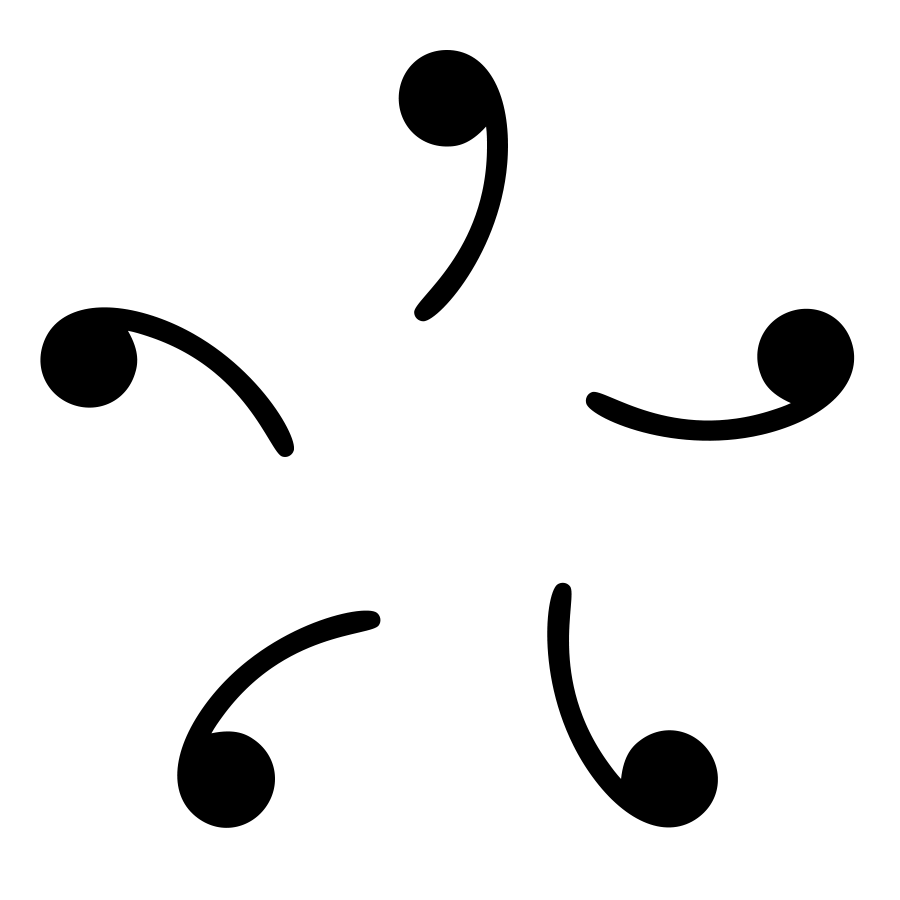
\includegraphics[width=0.9in]{logo.png}}}
\end{picture}
\vspace{-3.5em}

\subsubsection*{Lecture problems}

\begin{minipage}{.70\textwidth}
  \begin{enumerate}
    \item (QI6) Three circles with radii 4, 5, and 9 have the same center. If $x\%$ of the area of the largest circle lies between the other two circles, what is $x$ to the nearest integer?
    \item (QI12) In the figure on the right (not drawn to scale), triangle $ABC$ is equilateral, triangle $DBE$ is isosceles with $EB = BD$, and the lines $l_1$ and $l_2$ are parallel. What is $m\angle FBE$?
    \item (QI14) A regular hexagon with area $28$ is inscribed in a circle. What would the area of a square inscribed in the same circle be?
  \end{enumerate}
\end{minipage}
\begin{minipage}{.30\textwidth}
  \begin{center}
  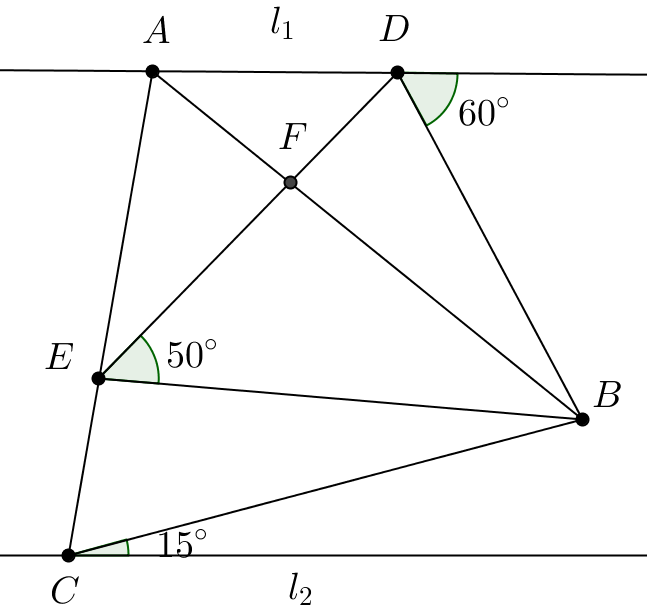
\includegraphics[width=.90\textwidth]{qi12.png}
  \end{center}
\end{minipage}

\begin{enumerate}
  \item[4.] (AI13) A circle is inscribed in a $2$ by $2$ square. Four squares are placed on the corners (the spaces between circle and square), in such a way that one side of the square is tangent to the circle, and two of the vertices lie on the sides of the larger square. Find the total area of the four smaller squares.
  \item[5.] Lines $l_1$ and $l_2$ are parallel. Points $A$ and $B$ are in $l_1$ and points $C$ and $D$ are in $l_2$ such that $A$ and $D$ are on opposite sides of line $BC$. Point $X$ is in between lines $l_1$ and $l_2$ such that $\angle BAX = 37\dg$ and $\angle XCD = 23\dg$. What is $m\angle AXC$?
  \item[6.] In a square, four semicircles centered on the midpoints of its sides are drawn inward. Find the total area of the regions common to two semicircles.
  \item[7.] The medians to the legs of an isosceles triangle are perpendicular to each other. If the base of the triangle is 4, find its area.
\end{enumerate}

\subsubsection*{Angles}

\begin{itemize}
  \item Circles make lots of angle relations, especially tangents to circles.
  \item Parallel lines make lots of equal angles, see problem 2.
  \item Don't be afraid to add additional lines, as in the sigma problem. 
  \item Draw large diagrams. Rule: if you cannot make any more markings, draw a larger diagram.
\end{itemize}

\subsubsection*{Areas}
\begin{itemize}
  \item For a triangle $ABC$ with side lengths $a, b, c$, altitudes to sides $BC$, $CA$, $AB$ $h_a, h_b, h_c$, angles $A, B, C$, semiperimeter $s$, inradius $r$ and circumradius $R$, its area is
$$[ABC] = \frac{ah_a}{2} = \frac12 ab \sin C = \sqrt{(s-a)(s-b)(s-c)} = rs = \frac{abc}{4R}.$$
  \item Similar figures with ratio $k$ have ratio of areas $k^2$: look at the trapezoid.
  \item Break down into smaller areas and then add and subtract them, like problems 1, 3, 6.
  \item Length chase. As in problems 4 and 7.
\end{itemize}

\end{document}
